\documentclass[hyperref,]{ctexart}
\usepackage{lmodern}
\usepackage{amssymb,amsmath}
\usepackage{ifxetex,ifluatex}
\usepackage{fixltx2e} % provides \textsubscript
\ifnum 0\ifxetex 1\fi\ifluatex 1\fi=0 % if pdftex
  \usepackage[T1]{fontenc}
  \usepackage[utf8]{inputenc}
\else % if luatex or xelatex
  \ifxetex
    \usepackage{xltxtra,xunicode}
  \else
    \usepackage{fontspec}
  \fi
  \defaultfontfeatures{Mapping=tex-text,Scale=MatchLowercase}
  \newcommand{\euro}{€}
\fi
% use upquote if available, for straight quotes in verbatim environments
\IfFileExists{upquote.sty}{\usepackage{upquote}}{}
% use microtype if available
\IfFileExists{microtype.sty}{%
\usepackage{microtype}
\UseMicrotypeSet[protrusion]{basicmath} % disable protrusion for tt fonts
}{}
\ifxetex
  \usepackage[setpagesize=false, % page size defined by xetex
              unicode=false, % unicode breaks when used with xetex
              xetex]{hyperref}
\else
  \usepackage[unicode=true]{hyperref}
\fi
\usepackage[usenames,dvipsnames]{color}
\hypersetup{breaklinks=true,
            bookmarks=true,
            pdfauthor={Jingwen Yang},
            pdftitle={环洱海旅拍},
            colorlinks=true,
            citecolor=blue,
            urlcolor=blue,
            linkcolor=magenta,
            pdfborder={0 0 0}}
\urlstyle{same}  % don't use monospace font for urls
\usepackage{graphicx,grffile}
\makeatletter
\def\maxwidth{\ifdim\Gin@nat@width>\linewidth\linewidth\else\Gin@nat@width\fi}
\def\maxheight{\ifdim\Gin@nat@height>\textheight\textheight\else\Gin@nat@height\fi}
\makeatother
% Scale images if necessary, so that they will not overflow the page
% margins by default, and it is still possible to overwrite the defaults
% using explicit options in \includegraphics[width, height, ...]{}
\setkeys{Gin}{width=\maxwidth,height=\maxheight,keepaspectratio}
\usepackage[normalem]{ulem}
% avoid problems with \sout in headers with hyperref:
\pdfstringdefDisableCommands{\renewcommand{\sout}{}}
\setlength{\emergencystretch}{3em}  % prevent overfull lines
\providecommand{\tightlist}{%
  \setlength{\itemsep}{0pt}\setlength{\parskip}{0pt}}
\setcounter{secnumdepth}{5}

\title{环洱海旅拍}
\author{Jingwen Yang}
\date{2018-08-01}

% Redefines (sub)paragraphs to behave more like sections
\ifx\paragraph\undefined\else
\let\oldparagraph\paragraph
\renewcommand{\paragraph}[1]{\oldparagraph{#1}\mbox{}}
\fi
\ifx\subparagraph\undefined\else
\let\oldsubparagraph\subparagraph
\renewcommand{\subparagraph}[1]{\oldsubparagraph{#1}\mbox{}}
\fi

\begin{document}
\maketitle

{
\setcounter{tocdepth}{2}
\tableofcontents
}
  今天本可爱一扫前日的阴霾,抱了一个环洱海旅拍一日团。同行的有三个乘客,除了我还有一对湖南来的夫妻,领队是个白族的年轻小哥哥。
  今天应该是白族的一个节日,我看家家门口都放着一坨香。
  上车的时候同行的大哥问领队这边是不是种了很多仙人掌,领队说路边有很多卖仙人掌果实的。我当时听了之后心里很开心,觉得这个仙人掌的果实肯定很好吃。结果中午吃完饭在去下一个地点的路上我突然顿悟,``仙人掌的果实''不就是``仙人果''嘛:smile:
。我一直没有把吃到的仙人果跟仙人掌联系起来,哈哈哈哈哈哈。
  今天难得出了太阳,天气倒是非常好,但是超级超级晒。小姐姐还穿了裙子,防晒霜不知道涂了几层。今天的命都是防晒霜,太阳镜,遮阳帽,水杯还有冲锋衣给的。
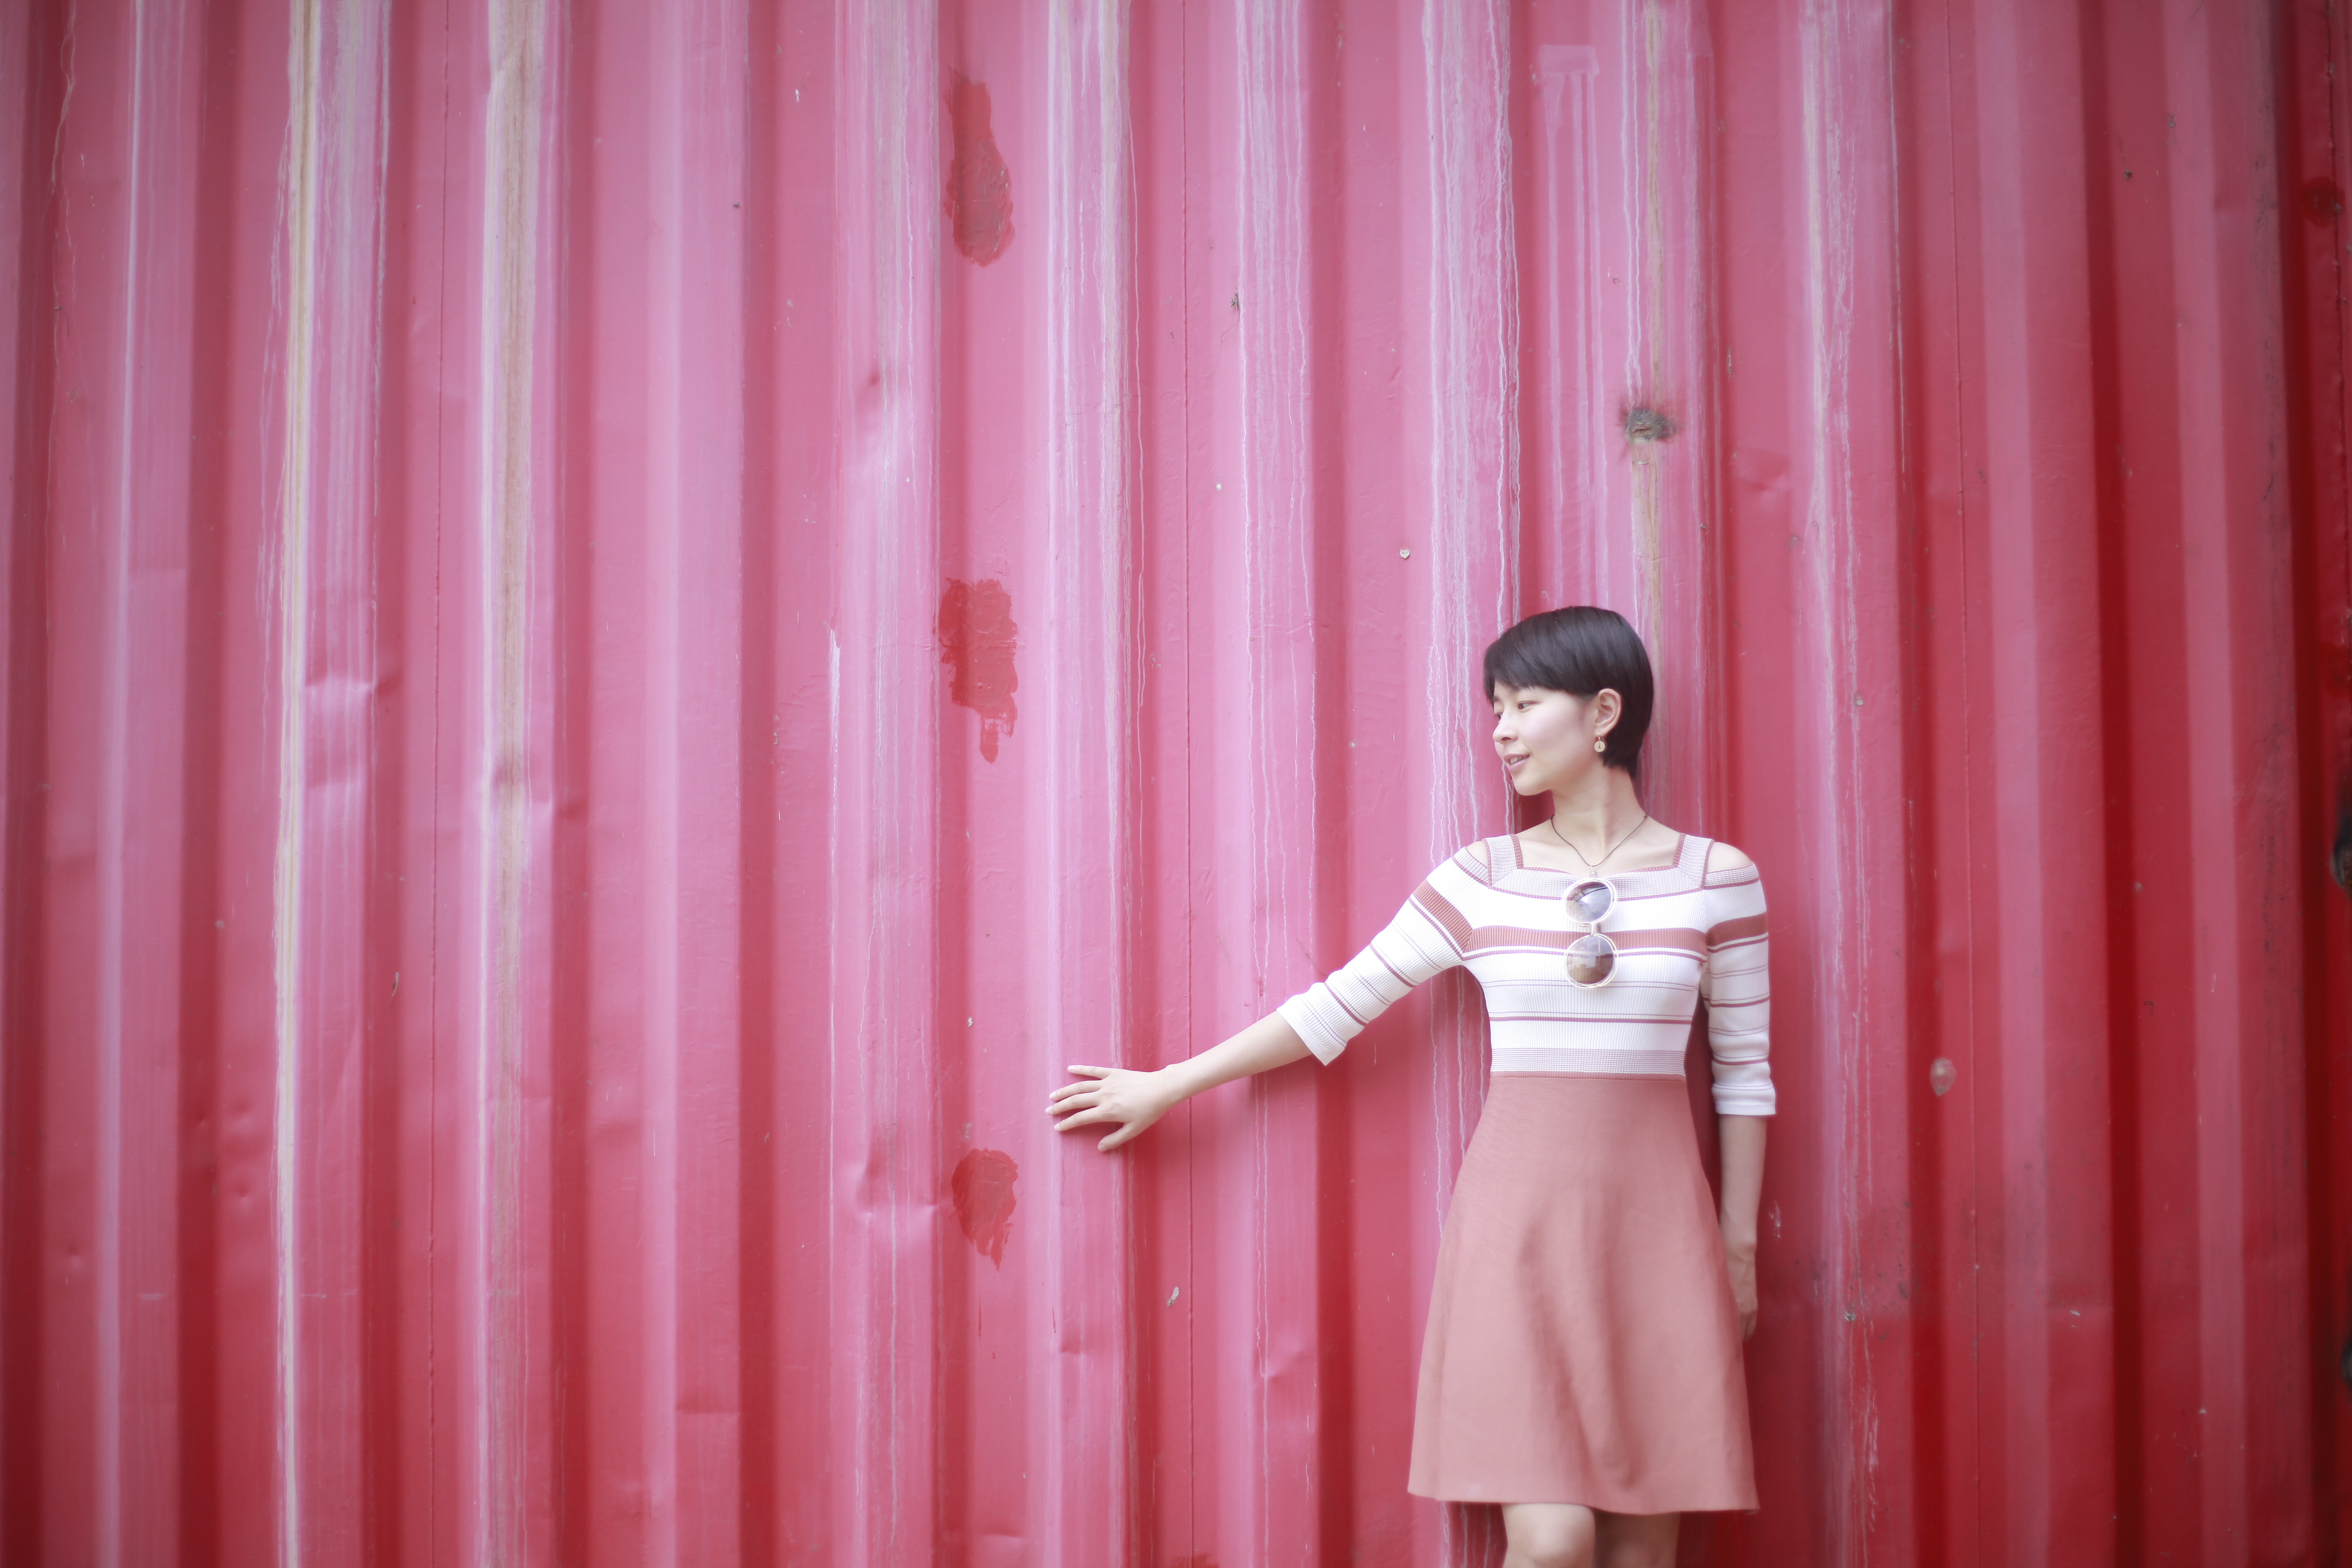
\includegraphics[width=0.8\textwidth,height=0.8\textwidth]{/post/2018-08-01-_files/2018-08-01 105811.jpg}
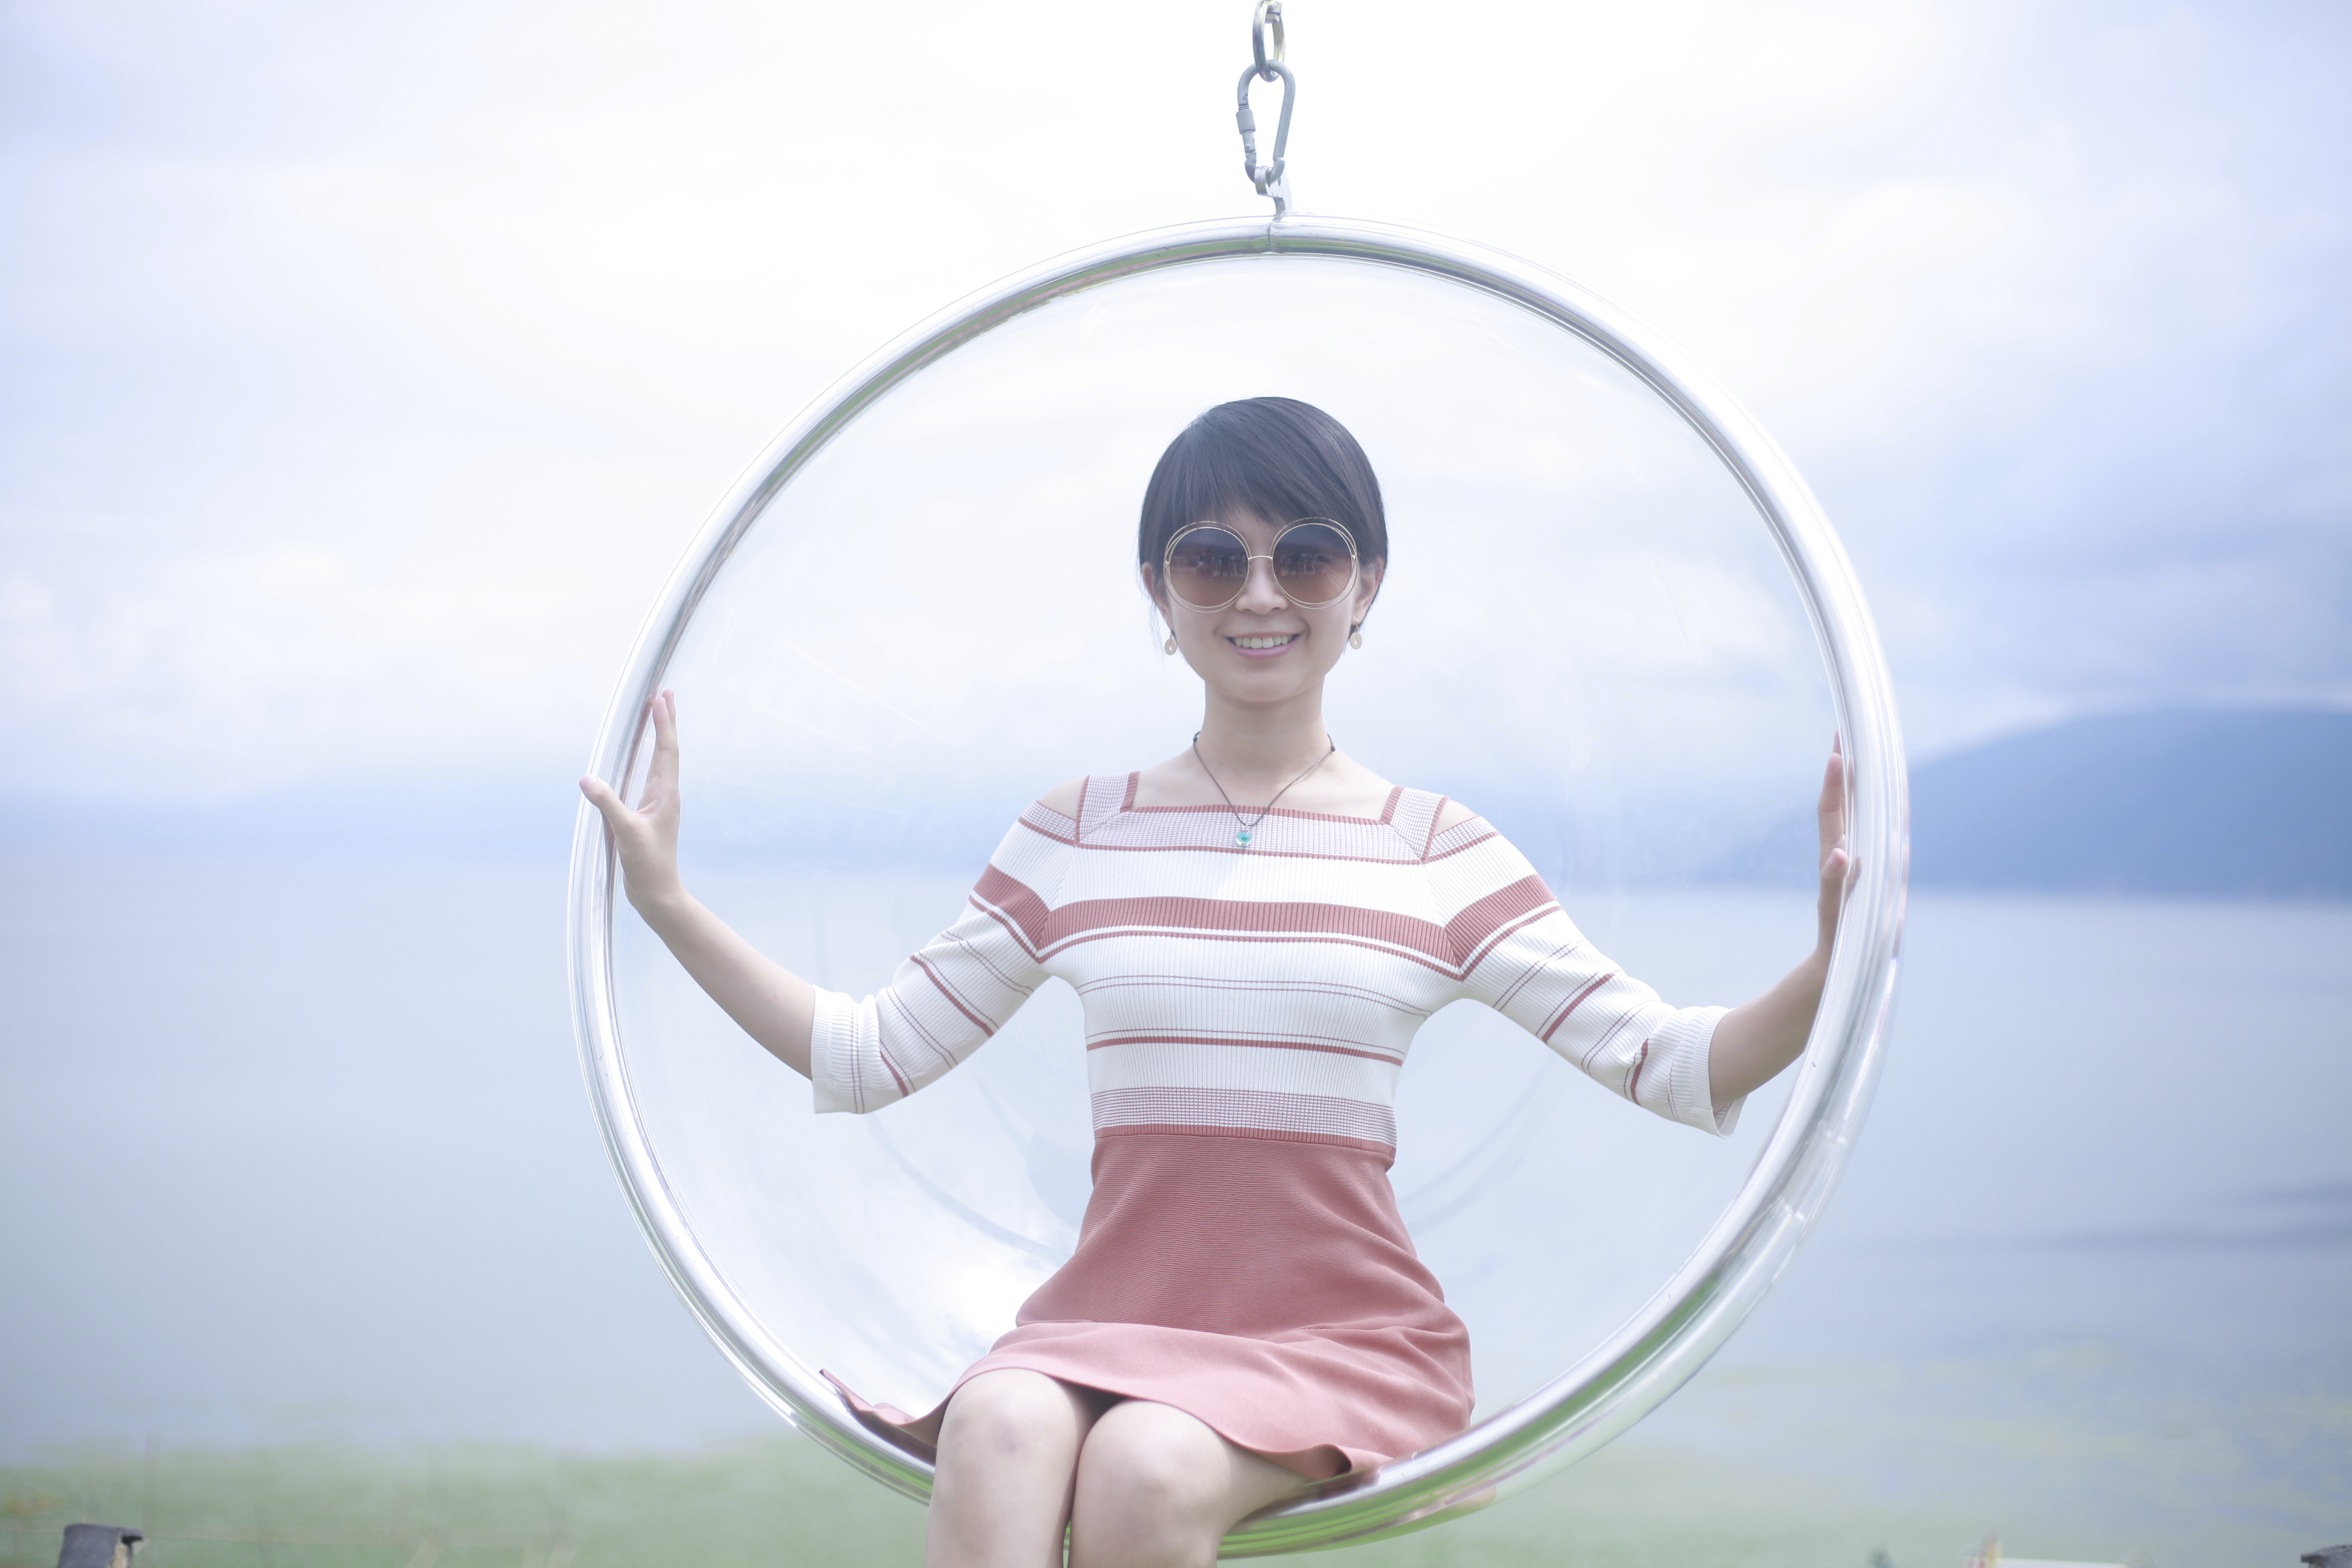
\includegraphics[width=0.8\textwidth,height=0.8\textwidth]{/post/2018-08-01-_files/2018-08-01 114842.jpg}
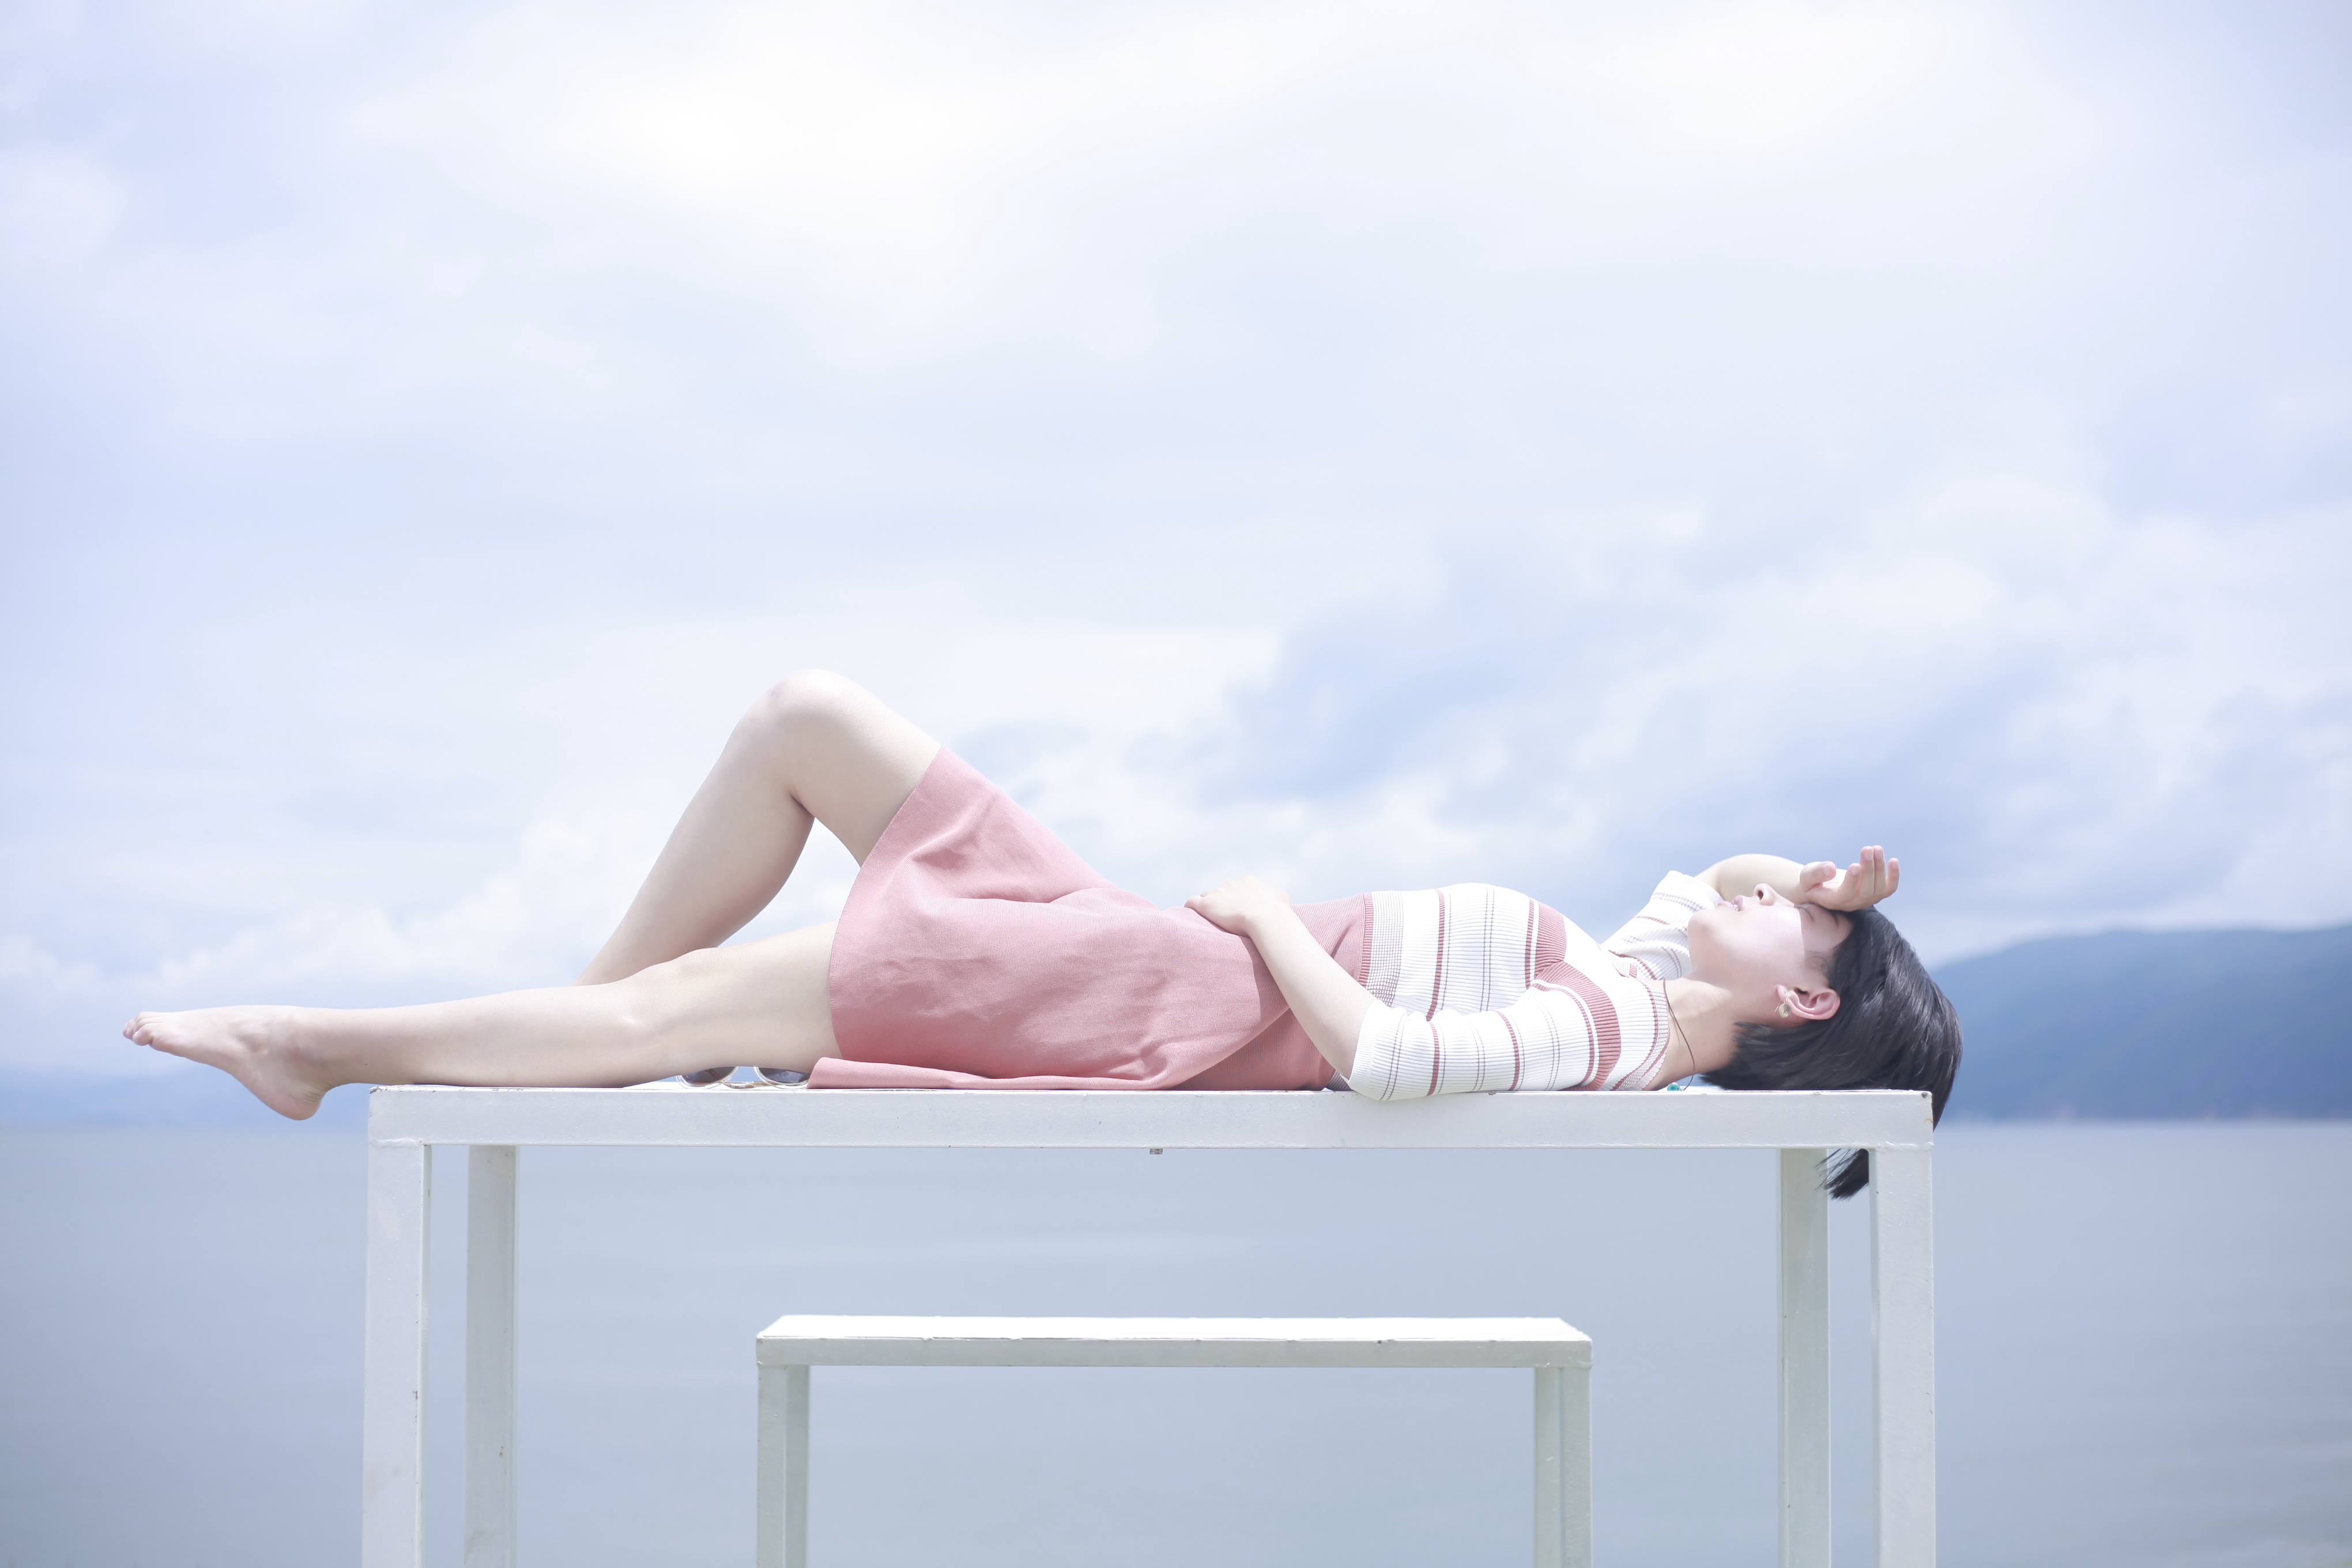
\includegraphics[width=0.8\textwidth,height=0.8\textwidth]{/post/2018-08-01-_files/2018-08-01 124637.jpg}
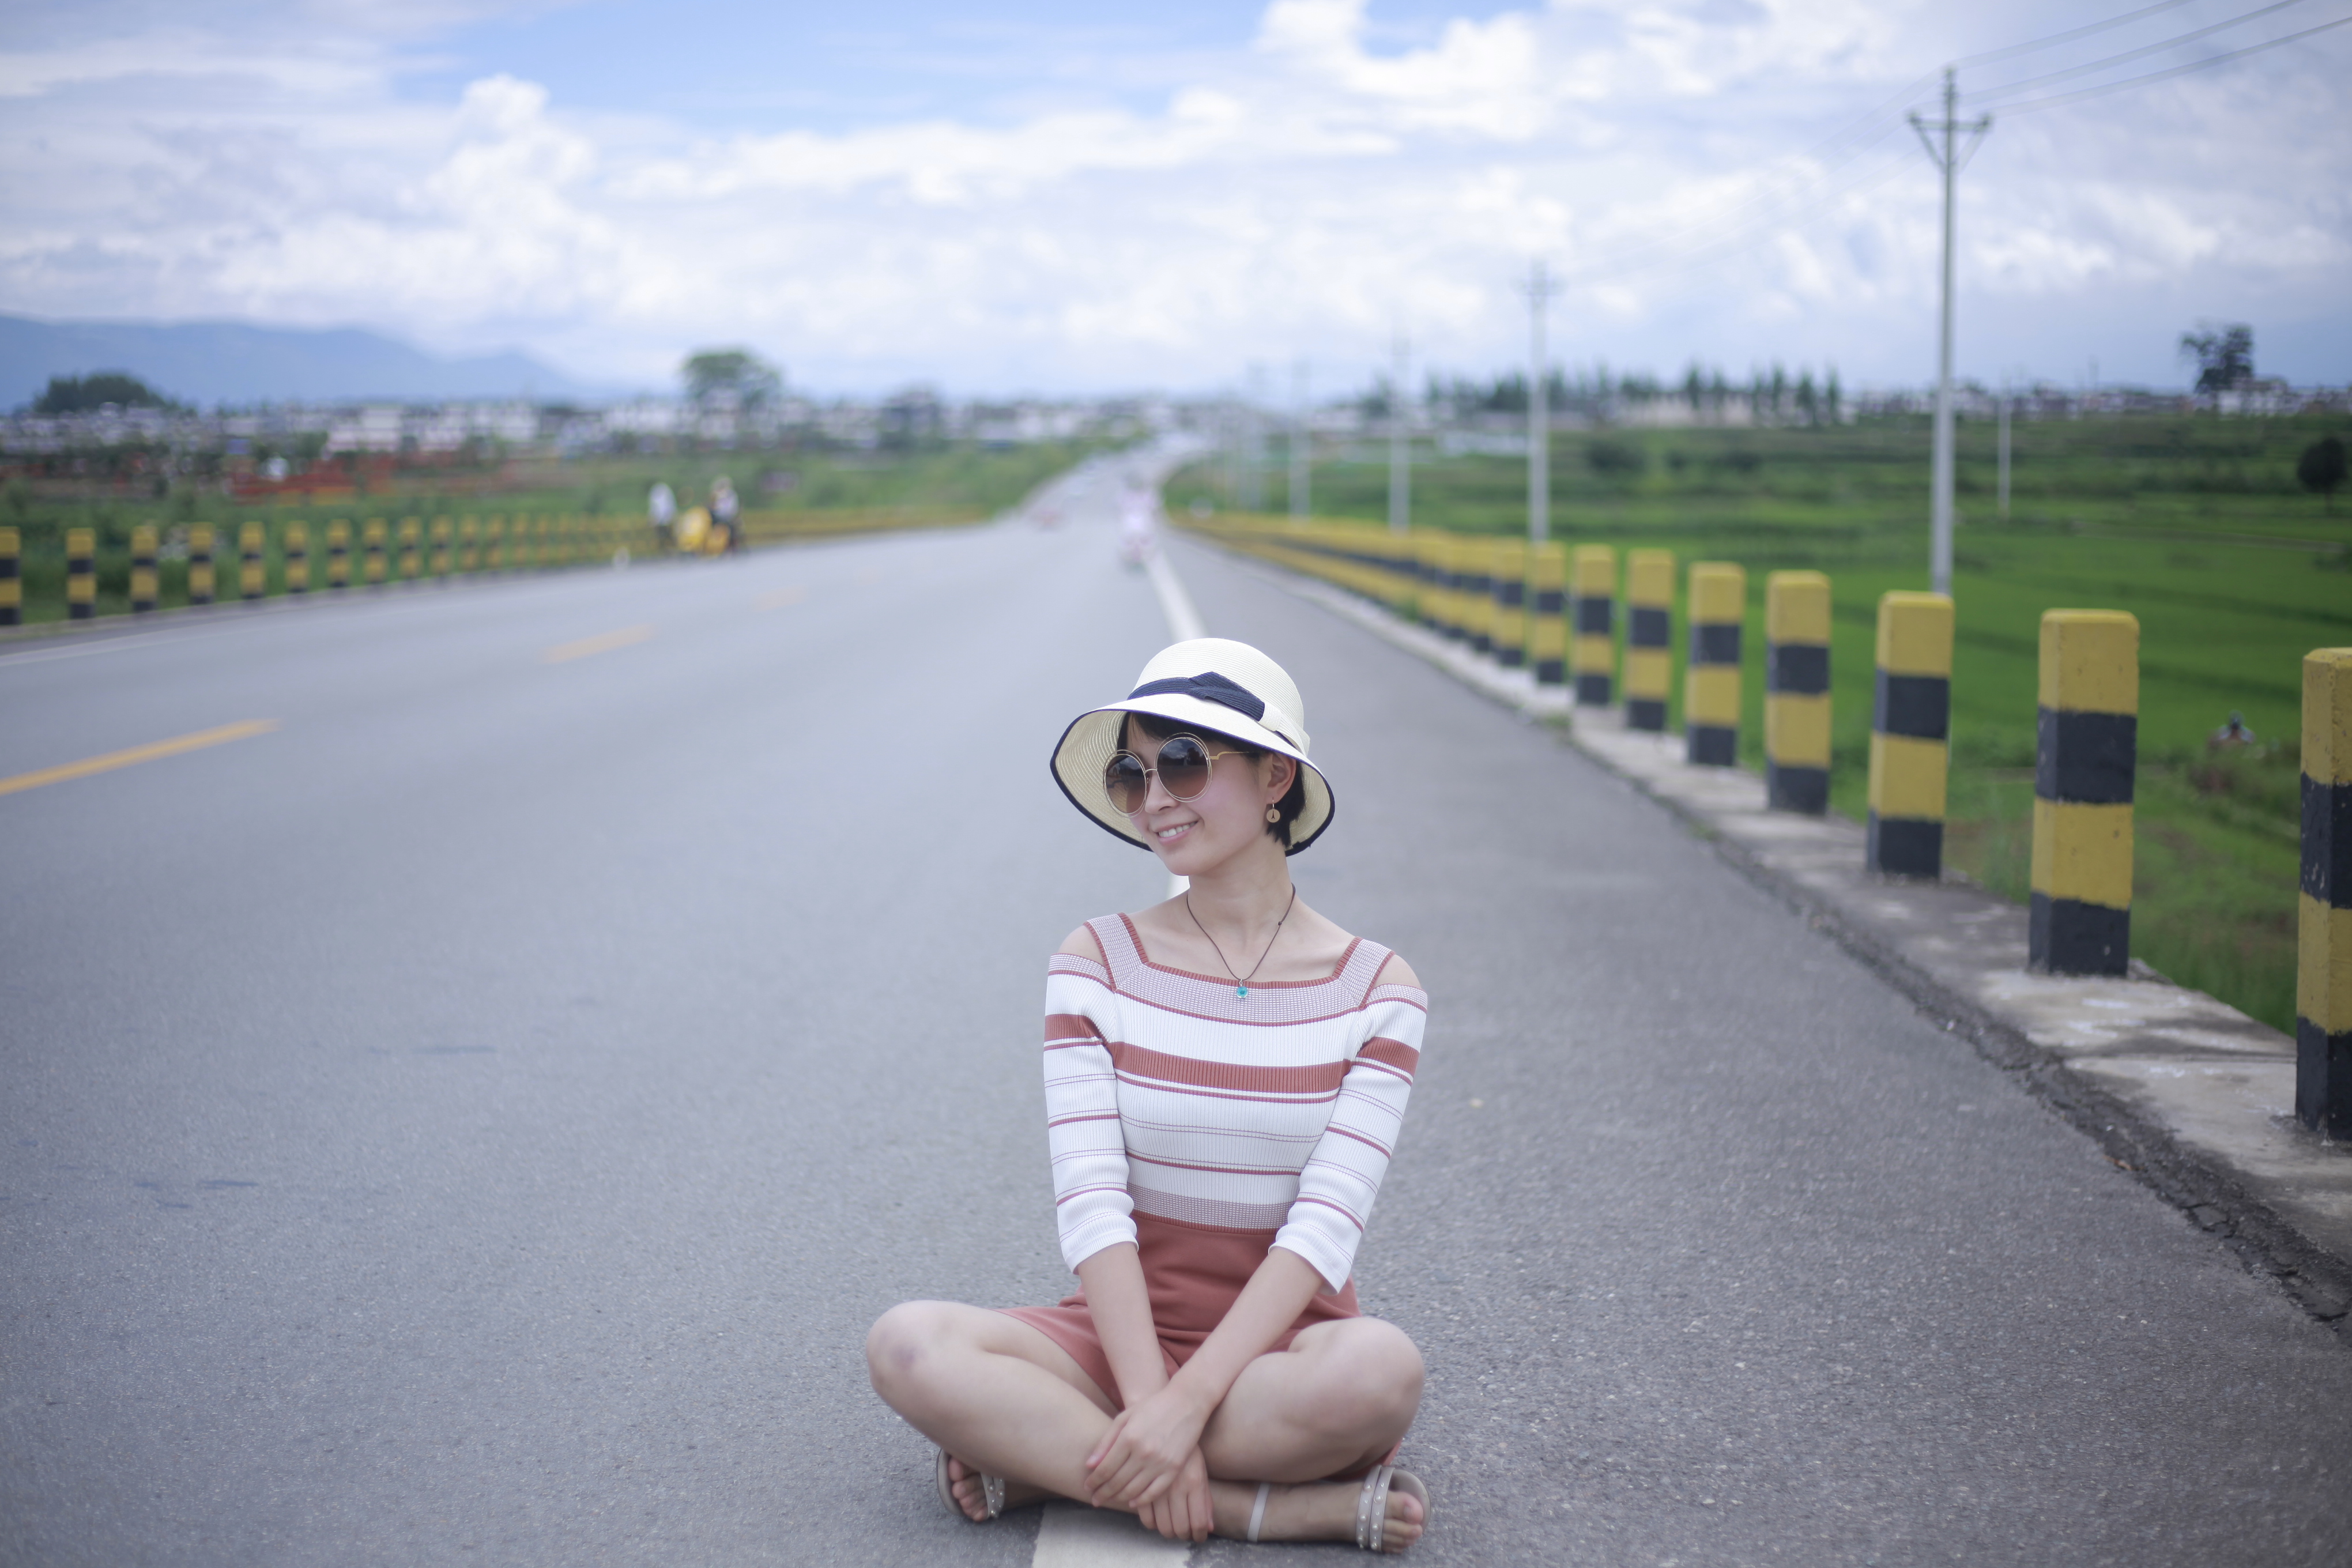
\includegraphics[width=0.8\textwidth,height=0.8\textwidth]{/post/2018-08-01-_files/2018-08-01 140856.jpg}
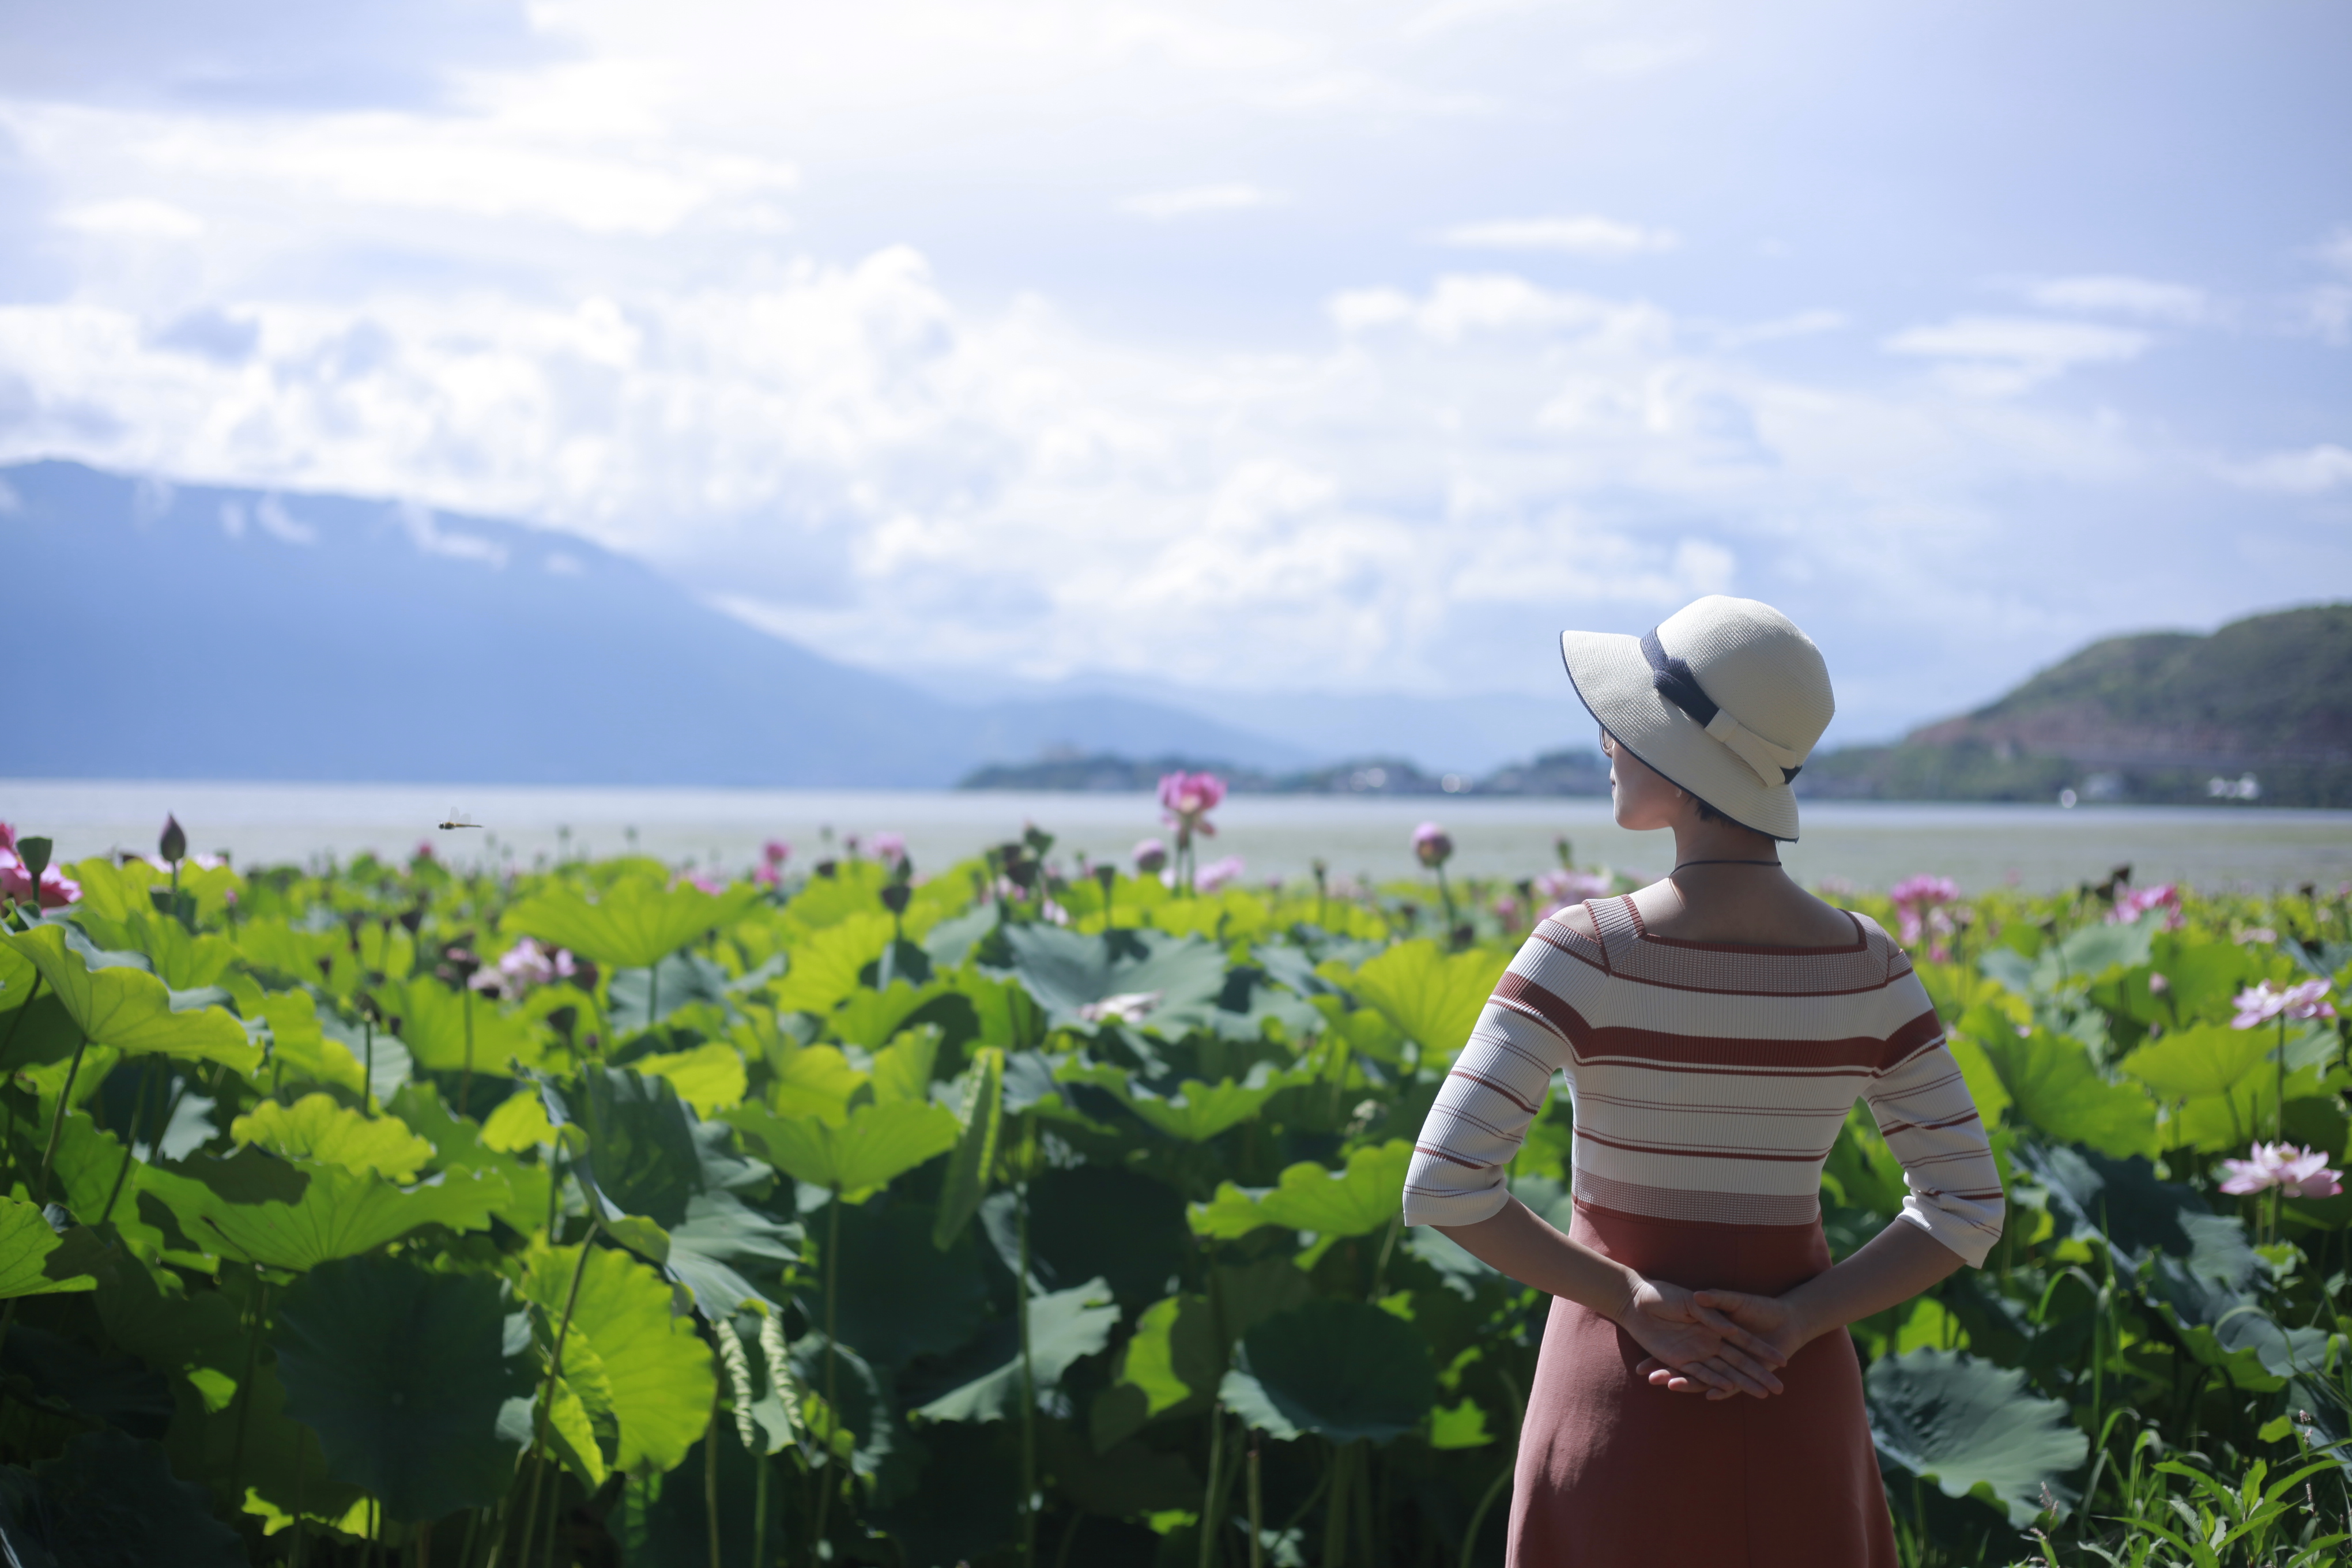
\includegraphics[width=0.8\textwidth,height=0.8\textwidth]{/post/2018-08-01-_files/2018-08-01 155910.jpg}
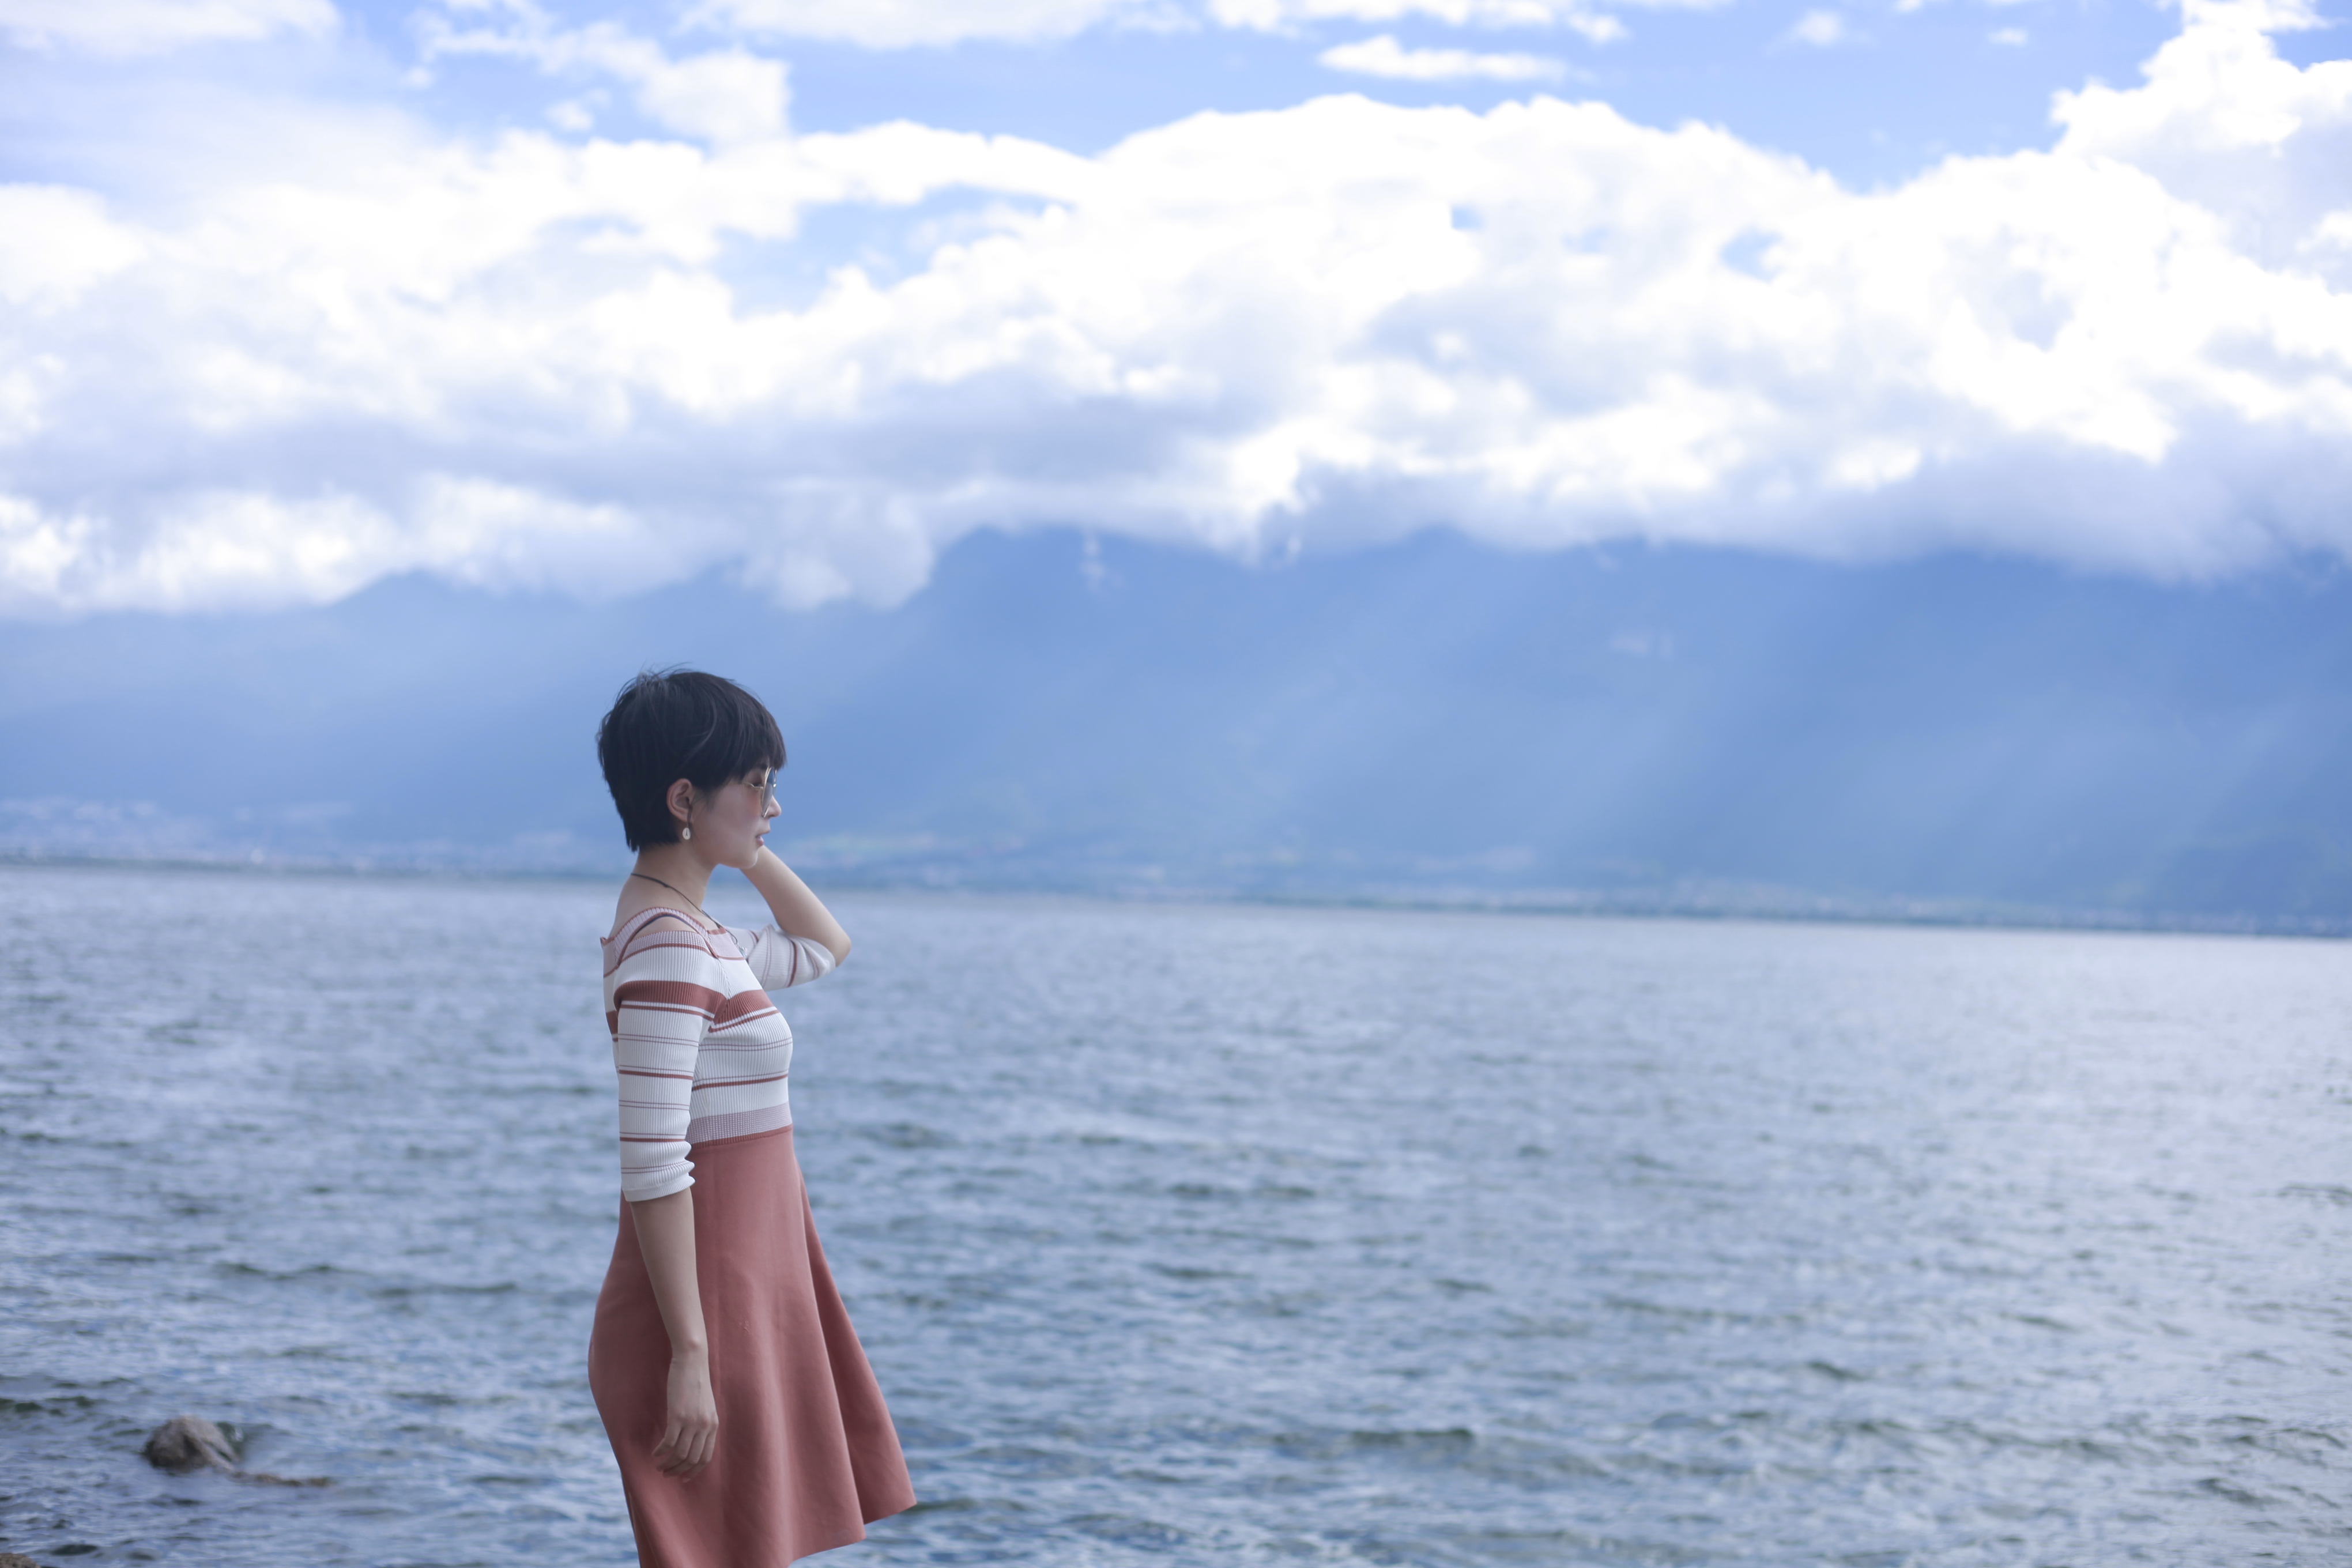
\includegraphics[width=0.8\textwidth,height=0.8\textwidth]{/post/2018-08-01-_files/2018-08-01 171520.jpg}

  午饭是在喜洲镇的一家小餐馆吃的,菜品中有黄焖鸡,我一口都没吃🌚,因为\sout{不可能会比在永平吃到的正宗的}。哈哈哈,主要原因还是辣。
  下午7点钟才回到古镇,我马上冲了个澡,想把涂的防晒全部洗掉。晚上到古镇觅食,磨磨蹭蹭,啥都没吃着,雨倒是下得挺大。淋倒是也没淋到,但是鞋子不防水,湿得很彻底。

\subsection{总结一下}

\begin{itemize}
\tightlist
\item
  今天很开心,环海东路的风景很漂亮,我还是很喜欢湖呀,海呀什么的。
\item
  很累,中午拍照片那会太阳很大,摘了太阳镜对着太阳,感觉脑袋要化了。
\item
  我今天很惊喜的发现,之前干的有点结珈的嘴巴,慢慢开始好了。开熏。
\end{itemize}

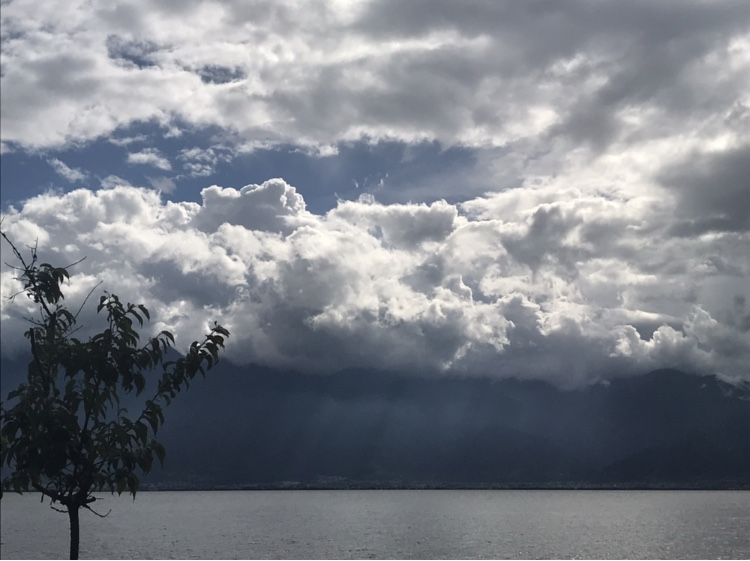
\includegraphics[width=0.8\textwidth,height=0.8\textwidth]{/post/2018-08-01-_files/IMG_6222.jpg}
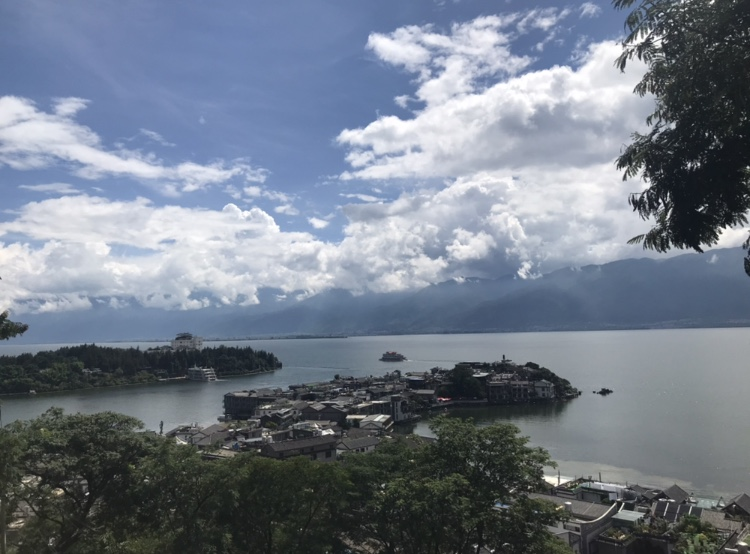
\includegraphics[width=0.8\textwidth,height=0.8\textwidth]{/post/2018-08-01-_files/IMG_6220.jpg}
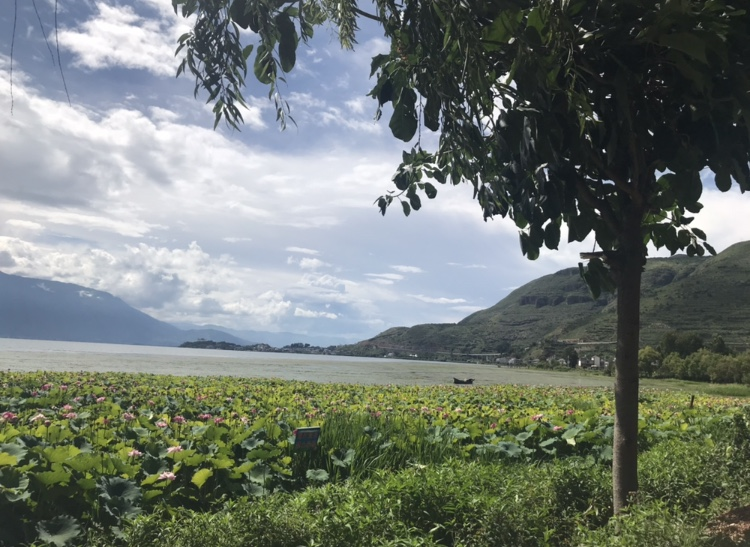
\includegraphics[width=0.8\textwidth,height=0.8\textwidth]{/post/2018-08-01-_files/IMG_6221.jpg}

\end{document}
